\chapter{Transformers}
\label{chap-transformers}

Transformers are a very recent family of architectures that have revolutionized fields like natural language processing (NLP), image processing, and multi-modal generative AI.


Transformers were originally introduced in the field of NLP in 2017, as an approach to process and understand human language. Human language is inherently sequential in nature (e.g., characters form words, words form sentences, and sentences form paragraphs and documents). Prior to the advent of the transformers architecture, recurrent neural networks (RNNs) briefly dominated the field for their ability to process sequential information (RNNs are described in Appendix \ref{chap-rnn} for reference). However, RNNs, like many other architectures, processed sequential information in an iterative/sequential fashion, whereby each item of a sequence was individually processed one after another. Transformers offer many advantages over RNNs, including their ability to process all items in a sequence in a \textit{parallel} fashion (as do CNNs).

% Transformers were originally introduced in the field of NLP, where they were used to model sequences of characters and words. There, transformers demonstrated significant improvements in the ability to model and understand complex and long data sequences. As a result, many texts present transformers as an alternative to the so-called recurrent neural nets (RNNs) for sequence modeling (RNNs are described in Chapter \ref{chap-rnn} for reference). In terms of the mechanics, however, transformer layers are \textit{parallel} processing machines, like convolutional layers, rather than sequential machines as RNNs are. This parallel nature is one of the main reasons for the effectiveness of transformers; and motivates our presentation below\footnote{The presentation of this chapter largely follows the book {\em Foundations of Computer Vision}, Transformer's Chapter, written by Philip Isola.}.

% Convolutional neural networks model patterns in space, and recurrent neural networks model patterns in time.  In both cases, the models look for locality, and by doing so the number of model parameters $\theta$ is kept relatively small, and can be made independent of the size $n$ of the dataset.  This makes CNNs and RNNs efficient to describe, and helps make them trainable.  However, these models struggle with patterns that are extended in space or time; for example, how do we efficiently account for the influence of words that appear early on in a sentence on much later parts?  In these models, when addressing such problems using long-range patterns, the gradients calculated during backpropagation often are too small to stably update the value of a weight.

Like CNNs, transformers factorize the signal processing problem into stages that involve independent and identically processed chunks. However, they also include layers that mix information across the chunks, called {\em attention layers,} so that the full pipeline can model dependencies between the chunks.

In this chapter, we describe transformers from the bottom up. We start with the idea of embeddings and tokens (Section~\ref{sec-embeddings}). We then describe the attention mechanism (Section~\ref{sec-qkv}). And finally we then assemble all these ideas together to arrive at the full transformer architecture in Section~\ref{sec-transformers}.

%%%%%%%%%%%%%%%%%%%%%%%%%%%%%%%%%%%%%%%%%%%%%%%%%%%%%%%%%%%%%%%%%%%%%%%%%%%%%
\section{Vector embeddings and tokens}
\label{sec-embeddings}

% - word2vec
%   - vector diagram: sweet savory sugar salt
%     paris – france + poland = warsaw
%   - vector addition
%   - cosine distance
%   - conditional PDF
%   - how to train for embeddings
%   - tokens (word fragments, sentences, subimages)

% concept of semantic embedding
Before we can understand the attention mechanism in detail, we need to first introduce a new data structure and a new way of thinking about neural processing for language.

% CHRIS' VERSION
The field of NLP aims to represent words with vectors (aka {\em word embeddings}) such that they capture semantic meaning. More precisely, the degree to which any two words are related in the `real-world' to us humans should be reflected by their corresponding vectors (in terms of their numeric values). So, words such as `dog' and `cat' should be represented by vectors that are more similar to one another than, say, `cat' and `table' are. Nowadays, it's also typical for every individual occurrence of a word to have its own distinct representation/vector. So, a story about a dog may mention the word `dog' a dozen times, with each vector being slightly different based on its context in the sentence and story at large.

To measure how similar any two word embeddings are (in terms of their numeric values) it is common to use {\em cosine similarity} as the metric:

% ORIG VERSION (i'd remove this)
%Consider the challenge of understanding human language.  Words that appear to be very different may have quite similar semantics to a listener, depending on the context in which they are used.  For example, ``sweet'' is to ``sugar'' as ``savory'' is to ``salt'', and it is desirable to be able to capture such semantic relationships by mapping words to numerical vectors, e.g., representing word $w$ with a $d$-dimensional vector $v_w$.  Such multidimensional vectors are typically termed as ``tokens'' in the transformers literature.

% \note{In language modeling, a token might represent a word, so that a sequence of tokens is a sentence. In computer vision, a token may correspond to an image patch, so that an array of tokens represents an image}. 

% CT: I'd remove this, too
%The tokenization of words (or other kinds of raw data) help capture the fact that some words statistically occur closer to other words in written text.  For example, ``quantum'' likely appears more often in the vicinity of ``physics'' than near ``weather,'' whereas ``rain'' and ``weather'' are more likely to occur in proximity to each other.

% older draft
% This is the goal, but not the mechanism. E.g., word2vec uses a skipgram model (which you discuss below). The intuition that is difficult for people (me, for instance) is why the thetas of that model make a good embedding. It would be great if you could motivate that. What's confusing is that these embeddings are not constructed by knowing semantic similarities, only by knowing co-occurrence patterns among tokens.


% ORIG VERSION (I'd remove this)
%One can use the so-called cosine similarity to encode the idea that, "closer" vectors can capture semantic similarities between words. In particular, if $u$ and $v$ are column vectors corresponding to two words, then the {\em cosine} similarity between them is given by
\begin{eqnarray}
  \frac{u^T v}{ |u|\, |v|\,} = \cos <u, v>
  \,,
\end{eqnarray}
% switch from \theta to \alpha to avoid confusion with \theta as used in rest of chapter.
where $|u|$ and $|v|$ are the lengths of the vectors, and $<u, v>$ is the angle between $u$ and $v$.  The cosine similarity is $+1$ when $u=v$, zero when the two vectors are perpendicular to each other, and $-1$ when the two vectors are diametrically opposed to each other.  Thus, higher values correspond to vectors that are numerically more similar to each other.
%closer semantic meaning of the words corresponding to the vectors.

While word embeddings -- and various approaches to create them -- have existed for decades, the first approach that produced astonishingly effective word embeddings was {\em word2vec} in 2012. This revolutionary approach was the first highly-successful approach of applying deep learning to NLP, and it enabled all subsequent progress in the field, including Transformers. The details of {\em word2vec} are beyond the scope of this course, but we note two facts: (1) it created a single word embedding for each distinct word in the training corpus (not on a per-occurrence basis); (2) it produced word embeddings that were so useful, many relationships between the vectors corresponded with real-world semantic relatedness. For example, when using {\em Euclidean distance} as a distance metric between two vectors, word2vec produced word embeddings with properties such as (where $v_{\tt word}$ is the vector for ${\tt word}$):



%The Euclidean distance between vector representations of words may also capture semantic meaning. To some extent, if $v_{\tt word}$ is the vector for ${\tt word}$, then
\begin{eqnarray}
  v_{\tt paris} - v_{\tt france} + v_{\tt italy} \approx v_{\tt rome}
\end{eqnarray}

This corresponds with the real-world property that Paris is to France what Rome is to Italy. This incredible finding existed not only for geographic words but all sorts of real-world concepts in the vocabulary. Nevertheless, to some extent, the exact values in each embedding is arbitrary, and what matters most is the holistic relation between all embeddings, along with how performant/useful they are for the exact task that we care about.

%since the idea might be that since the capital city of France is Paris, then the vector representations may capture the fact that the capital city of Italy is Rome.

% how good is an embedding
% This is one of the most common methods for computing embeddings, but not the only one. It's also worth mentioning that this method assigns the same embedding to a word independent of context; e.g., it does not solve the disambiguation problem for "bank" between "river bank" and "bank audit".


% The mapping of a word to a semantically meaningful vector is known as a {\em word embedding}, and is often referred to in the field as {\em word2vec}, following one of the early methodologies.  How good is a given embedding?  This can be tricky, because early methods assign the same embedding to a word independent of context.  For example, the word ``bank'' has very different meaning when used as ``river bank'' versus ``bank audit.''



%there are common methods by which good embeddings are obtained.

For example, an embedding may be considered good if it accurately captures the conditional probability for a given word to appear next in a sequence of words.  You probably have a good idea of what words might typically fill in the blank at the end of this sentence:
\begin{quote}
  After the rain, the grass was \underline{\hspace*{12ex}}
\end{quote}
Or a model could be built that tries to correctly predict words in the middle of sentences:
\begin{quote}
  The child fell \underline{\hspace*{12ex}} during the long car ride
\end{quote}
The model can be built by minimizing a loss function that penalizes incorrect word guesses, and rewards correct ones. This is done by training a model on a very large corpus of written material, such as all of Wikipedia, or even all the accessible digitized written materials produced by humans.

% skip-gram model

% The skip-gram model gives an explicit conceptual example of this approach, using an objective function $J(\theta)$ that is based on the conditional probability $p(w_{t+j}|w_t)$ for word $w_{t+j}$ to appear $j$ words away from the word $w_t$ at location $t$ in a corpus of words.  Specifically, the objective function to be minimized is the average of the logarithms of the conditional probabilities:
% \begin{eqnarray}
%   J(\theta) = - \frac{1}{T} \sum_{t=1}^T \ \ \ \ \sum_{|j|\leq c, j\neq 0} \log \ p(w_{t+j}|w_t)
%   \,,
% \end{eqnarray}
% where $w_1, w_2, \cdots w_T$ is the sequence of training words, and $c$ is the maximum ``skip'' distance being considered.  The conditional probabilities are determined by a softmax over the vector embeddings:
% \begin{eqnarray}
%   p(w_{t+j}|w_t) = \frac{\exp\left( v_{w_{t+j}}^T v_{w_j} \right)}{ \sum_{w} \exp\left( v_w^T v_w \right) }
%   \,,
% \end{eqnarray}
% where the denominator normalizes the softmax output to be between zero and one, and the sum is over all the $k$ words in the vocabulary.  In its simplest form, the $d$-dimensional vector $v_{w}$ embedding word $w$ may be computed through a simple matrix multiplication
% \newcommand*{\vertbar}{\rule[-1ex]{0.5pt}{2.5ex}}
% \newcommand*{\horzbar}{\rule[.5ex]{2.5ex}{0.5pt}}
% \begin{eqnarray}
%   v_w = \underbrace{
%     \left[
%       \begin{array}{cccc}
%         \vertbar  & \vertbar  &        & \\
%         v_{w_{1}} & v_{w_{2}} & \ldots & \\
%         \vertbar  & \vertbar  &        &
%       \end{array}
%       \right]
%   }_{W^T}
%   \underbrace{
%     \left[
%       \begin{array}{c}
%         0      \\
%         0      \\
%         \vdots \\
%         1      \\
%         0      \\
%         \vdots
%       \end{array}
%       \right]
%   }_{I(w)}
%   \,,
% \end{eqnarray}
% where $I(w) \in \R^{k\times 1}$ is the one-hot encoding of word $w$, and the weight matrix $W \in \R^{k\times d}$ (not to be confused with word $w$) maps words to vector embeddings, by virtue of each column of $W^T$ being the vector embedding of a particular word.  More complex models for encoding words into vectors can of course be employed; generally this is done using a multi-layer neural network, where $\theta$ captures all of the model parameters employed for the encoding model.
% W = d x k (so W^T is k x d)

% computational difficulty
% Note that the skip-gram model is elegant but overly simplistic.  In particular, in the form presented, this model is unfortunately impractical to train because computing the derivative of the logarithm of $p(w_{t+j}|w_t)$ entails a cost proportional to the size of the vocabulary, that can have millions of terms.  However, in practice it is reasonable to prune the set of words that are included in the conditional probability calculation, because there may be a-priori information about which words are very unlikely or more likely to be relevant.

% tokens
% Moreover, in general it is desirable to build vector embeddings not just for words, but instead for {\em tokens}.  For language models, tokens may be subparts of words, such as common groupings of characters that represent phonemes.  Also, vector embeddings are useful for a wide range of data beyond text.  Modern machine learning analyses of images, audio, and many other systems (robot dynamics!) now often begin with building representations of the data using vectorized tokens.


While we will not dive into the full details of {\em tokenization}, the high-level idea is straightforward: the individual inputs of data that are represented and processed by a model are referred to as {\em tokens}. And, instead of processing each word as a whole, words are typically split into smaller, meaningful pieces (akin to syllables). Thus, when we refer to tokens, know that we're referring to each individual input, and that in practice, nowadays, they tend to be sub-words (e.g., the word `talked' may be split into two tokens, `talk' and `ed').

%%%%%%%%%%%%%%%%%%%%%%%%%%%%%%%%%%%%%%%%%%%%%%%%%%%%%%%%%%%%%%%%%%%%%%%%%%%%%
\section{Query, key, value, and attention}
\label{sec-qkv}

% - query, key, value
%
%   - dict storing foods, with keys pizza, apple, sandwich, donut, chili, burito, sushi, hamburger, ...
%   - goal is to look up a food based on something more general, e.g., "convenient" or "spicy"
%   - need way to learn unstructured relationships.
%   - query q = column vector, K = matrix of keys
%   - attention distribution alpha = softmax(q^T K)
%   - attention(q,K,v) = softmax(q^T K) . v
%   - let d_k be the dimension of each key, then to keep gradients well-sized, do
%     attention(q,K,v) = softmax(q^T K / sqrt{d_k}) . v

% We have seen how CNN and RNN structures model spatial patterns in images and causal sequences in temporal data.  Suppose we want to model more general patterns that have neither spatial or temporal regularity, but instead are much more complex.  

Attention is a strategy for processing global information efficiently, focusing just on the parts of the signal that are most salient to the task at hand.\note{What we present below is the so-called ``dot-product attention'' mechanism; there can be other variants that involve more complex attention functions}

% dictionary setting
It might help our understanding of the ``attention'' mechanism to think about a dictionary look-up scenario. Consider a dictionary with keys $k$ mapping to some values $v(k)$. For example, let $k$ be the name of some foods, such as {\tt pizza}, {\tt apple}, {\tt sandwich}, {\tt donut}, {\tt chili}, {\tt burrito}, {\tt sushi}, {\tt hamburger}, $\ldots$.   The corresponding values may be information about the food, such as where it is available, how much it costs, or what its ingredients are.

% semantic lookup challenge
Suppose that instead of looking up foods by a specific name, we wanted to query by cuisine, e.g., ``{\tt mexican}'' foods. Clearly, we cannot simply look for the word ``{\tt mexican}'' among the dictionary keys, since that word is not a food.
% lookup using cosine similarity
What does work is to utilize again the idea of finding ``similarity" between vector embeddings of the query and the keys. The end result we'd hope to get, is a probability distribution over the foods, $p(k|q)$ indicating which are best matches for a given query $q$. With such a distribution, we can look for keys that are semantically close to the given query.

More concretely, to get such distribution, we follow these steps: First, embed the word we are interested in (``{\tt mexican}'' in our example) into a so-called query vector, denoted simply as $q \in \R^{d_k \times 1}$ where $d_k$ is the embedding dimension.

Next, suppose our given dictionary has $n$ number of entries/entries, we embed each one of these into a so-called key vector. In particular, for each of the $j^{th}$ entry in the dictionary, we produce a $k_j \in \R^{d_k\times 1}$ key vector, where $j=1,2,3, \dots, n.$

We can then obtain the desired probability distribution using a softmax (see Chapter~\ref{chap-neural_networks}) applied to the inner-product between the key and query:

\begin{equation*}
  p(k|q) ={softmax}\left(
  [q^T k_1; q^T k_2; q^T k_3; \dots, q^T k_n]
  \right)
\end{equation*}

This vector-based lookup mechanism has come to be known as ``attention'' in the sense that $p(k|q)$ is a conditional probability distribution that says how much attention should be given to the key $k_j$ for a given query $q$.

% In particular, let $d_k$ denote the size of the vocabulary, , and $\bar{k} \in \R^{d_k\times n_k}$ be a matrix of the one-hot encodings of all the keys.  And suppose we encode these as vectors using the so-called key-weight matrix $W_k \in R^{d_k \times d} $, such that
% \begin{eqnarray}
%   K = W^T \bar{k}
% \end{eqnarray}
% is a $\R^{ d \times n_k}$ matrix of vector encodings of the keys.  

% Then given the $\R^{d\times 1}$ encoding $Q = W^T q$ for query $q \in \R^{n_k\times 1}$ (which is a one-hot encoding of a word) similarly, we can lookup semantically close keys by computing the $R^{n_k \times 1}$ vector $Q^TK$.

% The elements of this vector give the cosine similarities between the query and the keys.  We then obtain the desired probability distribution using a softmax (see Chapter~\ref{chap-neural_networks}) applied to the cosine similarity vector:
% \begin{eqnarray}
%   p(k|q) = \text{softmax}\left( Q^T K \right)
%   \,.
% \end{eqnarray}

% attention mechanism



In other words, the conditional probability distribution $p(k | q)$ gives the ``attention weights,'' and the weighted average value
\begin{eqnarray}
  \sum_j p(k_j|q)\ v_j
  % \\
  % &=& \text{softmax}\left(Q^T K \right)\ v(k)
\end{eqnarray}
is the ``attention output.''

The meaning of this weighted average value may be ambiguous when the values are just words.  However, the attention output really becomes meaningful when the value are projected in some semantic embedding space (and such projection are typically done in transformers via learned embedding weights).

The same weighted-sum idea generalizes to multiple query, key, and values. In particular, suppose there are $n_q$ number of queries, $n_k$ number of keys (and therefore $n_k$ number of values), one can compute an attention matrix

\begin{eqnarray}A = \begin{bmatrix}
    \text{softmax}\left( \begin{bmatrix}
                           q_1^\top k_1 & q_1^\top k_2 & \cdots & q_1^\top k_{n_k}
                         \end{bmatrix} / \sqrt{d_k} \right) \\
    \text{softmax}\left( \begin{bmatrix}
                           q_2^\top k_1 & q_2^\top k_2 & \cdots & q_2^\top k_{n_k}
                         \end{bmatrix} / \sqrt{d_k} \right) \\
    \vdots &                                                                     \\
    \text{softmax}\left( \begin{bmatrix}
                           q_{n_q}^\top k_1 & q_{n_q}^\top k_2 & \cdots & q_{n_q}^\top k_{n_k}
                         \end{bmatrix} / \sqrt{d_k} \right)
  \end{bmatrix}
\end{eqnarray}\label{eq:xfm_softmax}

Here, $\text{softmax}_j$ is a softmax over the $n_k$-dimensional vector indexed by $j$, so in Eq.~\ref{eq:xfm_softmax} this means a softmax computed over keys.  In this equation, the normalization by $\sqrt{d_k}$ is done to reduce the magnitude of the dot product, which would otherwise grow undesirably large with increasing $d_k,$ making it difficult for (overall) training.

Let $\alpha_{ij}$ be the entry in $i$th row and $j$th column in the attention matrix $A$. Then $\alpha_{ij}$ helps answer the question "which tokens $x^{(j)}$ help the most with
predicting the corresponding output token $y^{(i)}$?" The attention output is given
by a weighted sum over the values:

$${y}^{(i)} = \sum_{j=1}^n  \alpha_{ij}
  v_{j}$$


%%%%%%%%%%%%%%%%%%%%%%%%%%%%%%%%%%%%%%%%
% \subsection{Towards language models with attention}
% % seq2seq with RNNs

% A {\em language model}, at its simplest level, predicts the next word to come in a sequence of words, given previous words in the sequence.  For example, consider a prompt and a response.  For example, say the prompt is a phrase in Japanese, ``ko re wa ii de wa nai,'' and the desired response is its translation into English.  One way to perform this translation task uses two RNN's in the form we previously saw in Section~\ref{sec-seq2seq_rnn}, where an encoder RNN generates a vector embedding of the prompt, then a decoder RNN generates the response given the final internal state of the encoder RNN:
% \begin{center}
%   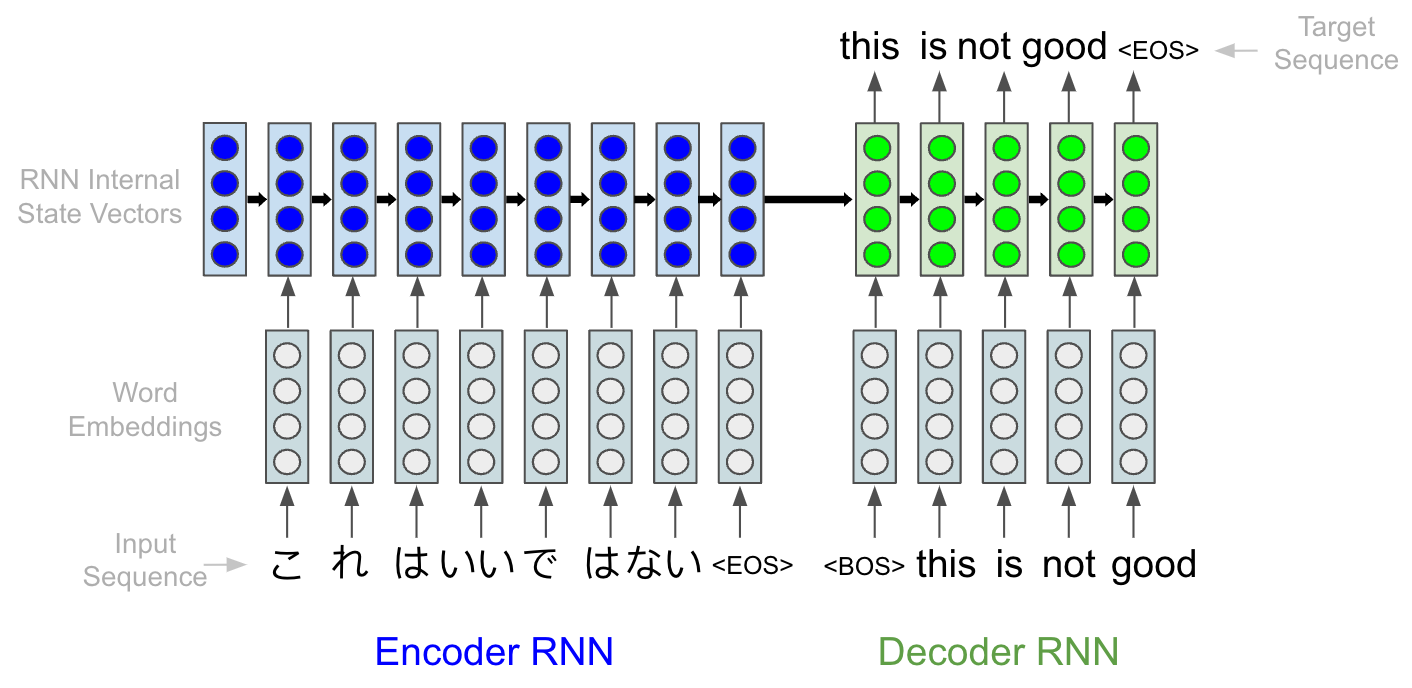
\includegraphics[width=5.5in]{figures/seq2seq-with-embeddings.png}
% \end{center}
% Each word is first turned into a vector embedding, then processed by the RNN.  The input sequence is the prompt, and the encoder RNN processes this input until it receives a special ``end of sequence'' (EOS) symbol.  The final state of the encoder RNN is then fed into the decoder RNN, which starts with the ``begin of sequence'' (BOS) symbol.  The decoder RNN is trained to output one word of the target sequence at each time step.  The output word at time $t$ is fed in as the input to the decoder RNN for time $t+1$, then the decoder RNN is used to generate the output word at time $t+1$.

% % problem with RNNs
% %
% % - need for complex patterns: towards multi-headed attention
% %
% %   - sentence that needs a long window
% %     Unlike the other white ducks in the pond, its feathers were _____
% %     Just like the other white ducks in the pond, its feathers were _____
% %
% %   - Not all words are important
% %     Judy needed to figure out how many pumpkins to buy for the party.
% %     Since twenty guests were coming and three could share one pumpkin, she decided to buy ______
% %
% %   - The important words may appear anywhere in the sentence
% %     Weather forcasts have clearly gotten much ______ since the since the game started 
% %     allowing magic users to abruptly change seasons in the fantasy world
% This can work pretty well for short prompts.  The challenge comes when the input sequence is long, because all the information about the prompt must be encoded in the final state of the encoder RNN.  And the state of an RNN typically becomes increasingly uncorrelated with a given input the further away it is in time.  For language translation, this is a pressing problem when the two languages have different grammar.  In Japanese, the sentiment of a sentence can be completely changed by the suffix added to the verb at the very end of the sentence.  This means that to accurately translate Japanese to English, the encoder RNN in our example needs to know both the initial and final Japanese words.  But the RNN will perform increasingly poorly as the input sentence gets longer.

% % seq2seq with attention
% Alternatively, an attention mechanism can be employed.  Conceptually, what we want is for the current state of the decoder RNN to be able to pay attention to a specific state vector of the encoder RNN, instead of just looking at the encoder RNN's final state.  For example, after outputting the word ``is,'' the decoder RNN in our Japanese translation scenario would want to know most about encoder RNN's state specifically at the word ``nai'' in the input, since that would generate the following English word in the output, ``not.''  We can accomplish this by employing the state of the encoder RNN as being both the keys and values, and letting the current state of the decoder RNN be the query, using this conceptual structure:
% \begin{center}
%   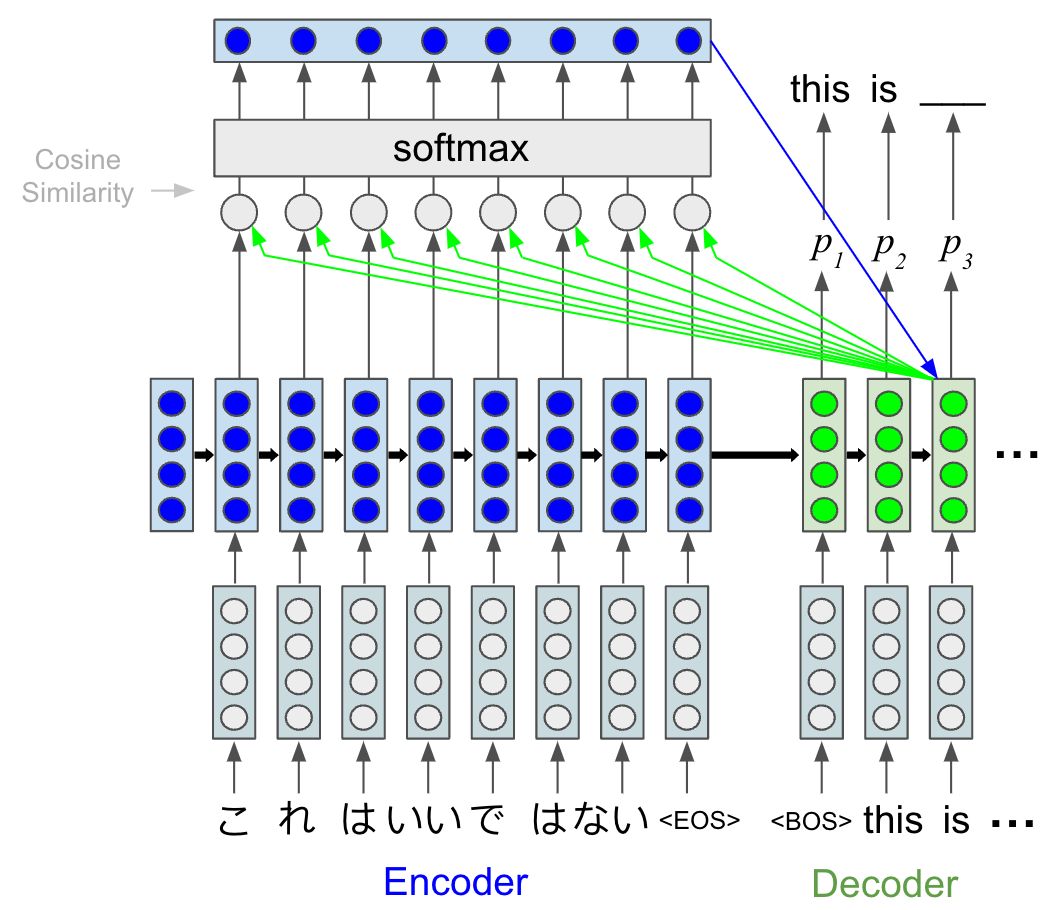
\includegraphics[width=4.615in]{figures/seq2seq-with-attention.png}
% \end{center}
% This is the conceptual structure of a seq2seq RNN with attention.  The top vector at the output of the softmax is the attention output, and this output is then used together with the decoder RNN's current state to produce the next output word.

% % patterns not based on spatial (CNN) or temporal (RNN) locality
% This usage of an attention mechanism bestows the RNNs with a kind of long-term memory, since generation of the output word can now utilize information from any word in the input sequence that is used to generate the attention output.  There are more sophisticated structures than the simple conceptual example given above.  For instance, the keys and values could use different vector embeddings, and an embedding could be applied to the values used to generate the attention output.  How the decoder employs the attention output to generate the next word can also be sophisticated.  And attention mechanisms are valuable not just for sequential data, but also for spatial data such as images.  Note that all of these embeddings and generation processes are generally neural networks that are trainable using back-propagation.  Actually training these embeddings can be difficult in practice, because of the large number of degrees of freedom, particularly as the number of keys and values grows.  But the main point to take away from this discussion is that attention mechanisms allows modeling of a far richer set of patterns than the temporally local RNN models, or even the spatially local CNN models, when applied to images.


% %%%%%%%%%%%%%%%%%%%%%%%%%%%%%%%%%%%%%%%%%%%%%%%%%%%%%%%%%%%%%%%%%%%%%%%%%%%%%




\subsection{Self Attention}
Self-attention is an attention mechanism where the keys, values, and queries are all generated from the same input.

At a very high level, typical transformer with self-attention layers maps $\mathbb{R}^{n\times d} \longrightarrow \mathbb{R}^{n\times d}$. In particular, the transformer takes in data (a sequence of tokens) $X\in \mathbb{R}^{n\times d}$ and for each token $x^{(i)}\in \mathbb{R}^{d\times 1}$, it computes (via learned projection, to be discussed in Section \ref{sec-learnedembedding}), a query $q_i \in \mathbb{R}^{d_q\times 1}$, key $k_{i} \in \mathbb{R}^{d_k\times 1}$, and value $v_{i} \in \mathbb{R}^{d_v\times 1}$. In practice, $d_q=d_k=d_v$ and we often denote all three embedding dimension via a unified $d_k.$\note{Note that $d_k$ differs from $d$: $d$ is the dimension of raw input token $\in \mathbb{R}^{d_q\times 1}$}

The self-attention layer then take in these query, key, and values, and compute a self-attention matrix
\begin{eqnarray}A = \begin{bmatrix}
    \text{softmax}\left( \begin{bmatrix}
                           q_1^\top k_1 & q_1^\top k_2 & \cdots & q_1^\top k_{n}
                         \end{bmatrix} / \sqrt{d_k} \right) \\
    \text{softmax}\left( \begin{bmatrix}
                           q_2^\top k_1 & q_2^\top k_2 & \cdots & q_2^\top k_{n}
                         \end{bmatrix} / \sqrt{d_k} \right) \\
    \vdots &                                                                   \\
    \text{softmax}\left( \begin{bmatrix}
                           q_{n}^\top k_1 & q_{n}^\top k_2 & \cdots & q_{n}^\top k_{n}
                         \end{bmatrix} / \sqrt{d_k} \right)
  \end{bmatrix}
\end{eqnarray}\label{eq:self_softmax}

Comparing this self-attention matrix with the attention matrix described in Equation \ref{eq:xfm_softmax}, we notice the only difference lies in the dimensions: since in self-attention, the query, key, and value all come from the same input, we have $n_q=n_k=n_v$, and we often denote all three with a unified $n$.

The self-attention output is then given by a weighted sum over the values:
$${y}^{(i)} = \sum_{j=1}^n  \alpha_{ij}
  v_{j}$$

This diagram below shows (only) the middle input token generating a query that is then combined with the keys computed with all tokens to generate the attention weights via a softmax. The output of the softmax is then combined with values computed from all tokens, to generate the attention output corresponding to the middle input token. Repeating this for each input token then generates the output.

% The idea is that for some input $x$, we generate a key $k = (W^k)^T x$ using a weight matrix $W^k$, a value $v = (W^v)^T x$ with weight matrix $W^v$, and a query using $(W^q)^T x$.  The attention mechanism then uses the attention function $\text{softmax}(q^T k)$ to determine which inputs are most relevant to a given $q$.  In the context of language translation example, this means that attention is used to determine which tokens (moving forward, let us think more generally, focusing on tokens instead of words) are most strongly related to each other.

\begin{center}
  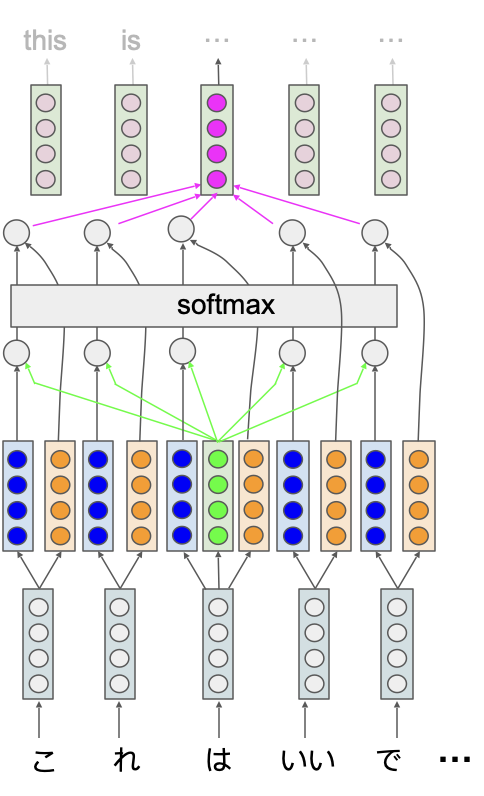
\includegraphics[width=2.615in]{figures/transformer-self-attention.png}
\end{center}



%  - output size same as input
%  - position encoding
%  - masking
\question{We have five colored tokens in the diagram above (gray, blue, organge, green, red). Could you read off the diagram the correspondence between the color and input, query, query, value, output? }

Note that the size of the output is the same as the size of the input.  Also, observe that there is no apparent notion of ordering of the input words in the depicted structure.  Positional information can be added by encoding a number for token (giving say, the token's position relative to the start of the sequence) into the vector embedding of each token.  And note that a given query need not pay attention to all other tokens in the input; in this example, the token used for the query is not used for a key or value.

% masking
More generally, a {\em mask} may be applied to limit which tokens are used in the attention computation.  For example, one common mask limits the attention computation to tokens that occur previously in time to the one being used for the query.  This prevents the attention mechanism from ``looking ahead'' in scenarios where the transformer is being used to generate one token at a time.

% % difference from RNN
% This single stage of self-attention is the principal component of a {\em transformer block}, and it is meaningfully different from an RNN: the transformer does not have a recurrent structure.  Thus, back-propagation-though-time does not need to be used, and the vanishing gradients problem of RNN's does not arise in the same way.  Moreover, all input tokens can be processed at once, instead of one at a time.  This means a transformer can be much faster to train than a comparable RNN: instead of requiring a number of training steps that grows linearly with the size of the input, the transformer can be trained in a single step, as long as sufficient computational resources are available for the parallel processing.

% multi-headed attention
Each self-attention stage is trained to have key, value, and query embeddings that lead it to pay specific attention to some particular feature of the input.  We generally want to pay attention to many different kinds of features in the input; for example, in translation one feature might be be the verbs, and another might be objects or subjects.  A transformer utilizes multiple instances of self-attention, each known as an ``attention head,'' to allow combinations of attention paid to many different features.

%%%%%%%%%%%%%%%%%%%%%%%%%%%%%%%%%%%%%%%%

\section{Transformers}
\label{sec-transformers}
A transformer is the composition of a number of transformer blocks, each of which has multiple attention heads. At a very high-level, the goal of a transformer block is to output a really rich, useful representation for each input token, all for the sake of being high-performant for whatever task the model is trained to learn.

Rather than depicting the transformer graphically, it is worth returning to the beauty of the underlying equations\footnote{The presentation here follows the notes by John Thickstun.}.





% formal definition
%
% Mathematical summary, following John Thickstun, but rewritten in 6.390 standard notation
% 6.390 conventions are that
% data input = d x n (each column is a data vector)
% superscript x^{(i)} indicates sample number
% NN output is W^T X
% need to include heads
%
% layer norm?
% residual connections?
%

%
\subsection{Learned embedding}\label{sec-learnedembedding}
For simplicity, we assume the transformer internally uses self-attention. Full general attention layers work out similarly.

Formally, a transformer block is a parameterized function $f_\theta$ that maps $\R^{n\times d}\rightarrow \R^{n\times d}$, where the input data $X \in \R^{n\times d}$ is often represented as a sequence of $n$ tokens, with each token $x^{(i)}\in \mathbb{R}^{d\times 1}.$


Three projection matrices (weights) $W_{q}, W_k, W_v$ are to be learned, such that, for each token $x^{(i)}\in \mathbb{R}^{d\times 1}$, we produce 3 distinct vectors: a query vector $q_i = W_q^T x^{(i)}$; a key vector $k_i = W_k^T x^{(i)}$; a value vector $v_i = W_v^T x^{(i)},$ all 3 of these vectors $\mathbb{R}^{d_k\times 1}$ and the learned weights $W_{q}, W_{k}, W_{v} \in \R^{d\times d_k}.$

If we stack these $n$ query, key, value vectors into matrix- form, such that $Q\in \mathbb{R}^{n\times d_k}$, $K\in \mathbb{R}^{n\times d_k}$, and $V\in \mathbb{R}^{n\times d_k},$ then we can more compactly write out the learned transformation from the sequence of input token $X$:
\begin{eqnarray*}
  Q &=& X W_{q}
  \\
  K &=& X W_{k}
  \\
  V &=& X W_{v}
\end{eqnarray*}
These $Q, K, V$ triple can then be used to produce one (self)attention-layer output. One such layer is called one "attention head".

One can have more than one "attention head", such that: the queries, keys, and values are embedded via encoding matrices:
\begin{eqnarray}
  Q^{(h)} &=& X W_{h,q}
  \\
  K^{(h)} &=& X W_{h,k}
  \\
  V^{(h)} &=& X W_{h,v}
\end{eqnarray}
and $W_{h,q}, W_{h,k}, W_{h,v} \in \R^{d\times d_k}$where $d_k$ is the size of the key/query embedding space, and $h \in \{1,\cdots,H\}$ is an index over ``attention heads.'' \note{for each attention-head $h$, we learn one set of $W_{h,q}, W_{h,k}, W_{h,v}$.}

We then perform a weighted sum over all the outputs for each head,
\begin{eqnarray}
  {u'}^{(i)} = \sum_{h=1}^H W^T_{h,c} \sum_{j=1}^{n} \alpha^{(h)}_{ij} V^{(h)}_j
  \,,
\end{eqnarray}

where $W_{h,c} \in \R^{d_k\times d},$ ${u'}^{(i)} \in \R^{d\times 1},$ the indices $i \in \{1,\cdots,n\}$ and $j \in \{1,\cdots,n\}$ are an integer index over tokens. \note{$V^{(h)}_j$ is the $d_k\times 1$ value embedding vector that corresponds to the input token $x^{j}$ for attention head $h$.}

This is then standardized and combined with $x^{(i)}$ using a $\text{LayerNorm}$ function (defined below) to become
\begin{eqnarray}
  {u}^{(i)} = \text{LayerNorm}\left(  x^{(i)} + {u'}^{(i)}; \gamma_1, \beta_1  \right)
\end{eqnarray}
with parameters $\gamma_1, \beta_1 \in \R^{d}$.

To get the final output, we follow the ``intermediate output then layer norm" recipe again. In particular, we first get the transformer block output ${z'}^{(i)}$ given by
\begin{eqnarray}
  {z'}^{(i)} = W_2^T \text{ReLU}\left( W_1^T u^{(i)} \right)
\end{eqnarray}
with weights $W_1\in \R^{d\times m}$ and $W_2\in \R^{m\times d}$.  This is then standardized and combined with $u^{(i)}$ to give the final output $z^{(i)}$:
\begin{eqnarray}
  {z}^{(i)} = \text{LayerNorm}\left(  u^{(i)} + {z'}^{(i)}; \gamma_2, \beta_2  \right)
  \,,
\end{eqnarray}
with parameters $\gamma_2, \beta_2 \in \R^{d}$.  These vectors are then assembled (e.g., through parallel computation) to produce $z\in \R^{n\times d}$.

The $\text{LayerNorm}$ function transforms a $d$-dimensional input $z$ with parameters $\gamma, \beta \in \R^d$ into
\begin{eqnarray}
  \text{LayerNorm}(z; \gamma, \beta) = \gamma \frac{z-\mu_z}{\sigma_z} + \beta
  \,,
\end{eqnarray}
where $\mu_z$ is the mean and $\sigma_z$ the standard deviation of $z$:
\begin{eqnarray}
  \mu_z &=& \frac{1}{d} \sum_{i=1}^d z_i
  \\
  \sigma_z &=& \sqrt{ \frac{1}{d} \sum_{i=1}^d (z_i-\mu_z)^2 }
  \,.
\end{eqnarray}
Layer normalization is done to improve convergence stability during training.

The model parameters comprise the weight matrices $W_{h,q}, W_{h,k}, W_{h,v}, W_{h,c}, W_1, W_2$ and the $\text{LayerNorm}$ parameters $\gamma_1, \gamma_2, \beta_1, \beta_2$.  A {\em transformer} is the composition of $L$ transformer blocks, each with its own parameters:
\begin{eqnarray}
  f_{\theta_L} \circ  \cdots \circ f_{\theta_2} \circ f_{\theta_1}(x) \in \R^{n\times d}
  \,.
\end{eqnarray}
The hyperparameters of this model are $d, d_k, m, H,$ and $L.$


% (where typically $d=512$, $d_k = 64$, $m=2048$, $H=8$, and $L\ge 6$.


%%%%%%%%%%%%%%%%%%%%%%%%%%%%%%%%%%%%%%%%
\subsection{Variations and training}

Many variants on this transformer structure exist.  For example, the $\text{LayerNorm}$ may be moved to other stages of the neural network.  Or a more sophisticated attention function may be employed instead of the simple dot product used in Eq.~\ref{eq:xfm_softmax}.  Transformers may also be used in pairs, for example, one to process the input and a separate one to generate the output given the transformed input.  Self-attention may also be replaced with cross-attention, where some input data are used to generate queries and other input data generate keys and values.  Positional encoding and masking are also common, though they are left implicit in the above equations for simplicity.

How are transformers trained?  The number of parameters in $\theta$ can be very large; modern transformer models like GPT4 have tens of billions of parameters or more.  A great deal of data is thus necessary to train such models, else the models may simply overfit small datasets.

Training large transformer models is thus generally done in two stages.  A first ``pre-training'' stage employs a very large dataset to train the model to extract patterns.  This is done with unsupervised (or self-supervised) learning and unlabelled data.  For example, the well-known BERT model was pre-trained using sentences with words masked.  The model was trained to predict the masked words.  BERT was also trained on sequences of sentences, where the model was trained to predict whether two sentences are likely to be contextually close together or not. The pre-training stage is generally very expensive.

The second ``fine-tuning'' stage trains the model for a specific task, such as classification or question answering.  This training stage can be relatively inexpensive, but it generally requires labeled data.



